\documentclass[12pt]{article}
\usepackage[papersize={5cm,5cm},tmargin=5mm,bmargin=5mm,lmargin=2mm,rmargin=5mm]{geometry}
\usepackage{tikz-network}

\begin{document}
\pagestyle{empty}
\thispagestyle{empty}
    \begin{figure}
        \centering
        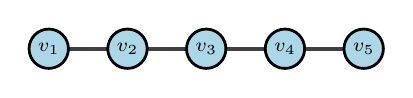
\begin{tikzpicture}
            \Vertex[x=-2, size=0.5, label=$v_1$]{A}
            \Vertex[x=-1, size=0.5, label=$v_2$]{B}
            \Vertex[x=0, size=0.5, label=$v_3$]{C}
            \Vertex[x=1, size=0.5, label=$v_4$]{D}
            \Vertex[x=2, size=0.5, label=$v_5$]{E}
            \Edge(A)(B)
            \Edge(B)(C)
            \Edge(C)(D)
            \Edge(D)(E)
        \end{tikzpicture}
    \end{figure}
\end{document}